\documentclass[a4paper,twoside,12pt,AutoFakeBold]{ctexart}
\newcommand\specialsectioning{\setcounter{secnumdepth}{-2}}
\specialsectioning
\usepackage[center]{titlesec}
\usepackage{indentfirst}
\setlength{\parindent}{2em}
\usepackage{fancyhdr}
\pagestyle{fancy}%fancy style
\usepackage{caption}
\fancyhf{}%清空页眉页脚
\fancyhead[LE,RO]{\thepage}%页码位置:偶数页居左,奇数页居右
\fancyfoot[RO,RE]{\textit{NEFU's seminar of Marxism}}% 设置页脚:在每页的右下脚以斜体显示书名
\usepackage{graphicx}
\setlength{\headheight}{15pt}%解决页眉warnings
\usepackage{amsmath}
\renewcommand{\headrulewidth}{0pt} % 页眉与正文之间的水平线粗细
\renewcommand{\footrulewidth}{0pt}
\usepackage{tcolorbox}%文本框宏包
\usepackage{changepage}%设置引用段落左右侧缩进

\usepackage{tabularx}
\usepackage{hyperref}%设置超链接
\usepackage{float}
\title{读书会记录}
\author{东北林业大学马克思主义研讨会\\
 吴云飞~编}
\date{2023-10}
\usepackage{perpage}
\MakePerPage{footnote}
\begin{document}
\maketitle
\newpage



\tableofcontents%目录

\newpage

\section{序言}

\begin{adjustwidth}{2em}{2em}
\qquad\fangsong 
本书是东北林业大学马克思主义经典著作研究与讨论会的一个内部记录,诸多观点与看法可能会欠缺专业性,因而这是一个非教学性质的内容记录。本书全部内容均来自我们的研讨会中的发言,如有雷同,纯属巧合,本书最终解释权归本研讨会与编辑组所有\footnote{已将本书的\LaTeX{}源代码置于编者的Github之中,供各位成员获取:\url{https://github.com/Imheaven233/Seminar-of-Marxism-of-NEFU}。}。

\end{adjustwidth}




\newpage

\section{第一期:《哲学的贫困》选读(1)}

\subsection{学习提示}\label{sec:1}

《哲学的贫困》是马克思针对蒲鲁东的《贫困的哲学》一书而写的一部论战性著作,以法文写成于1847年上半年,并于同年7月在布鲁塞尔和巴黎出版。

该著作分为两个部分,即第一章和第二章。第一章的讨论针对蒲鲁东为“工资平等”的社会主义所作的经济学论证,揭示这种论证尚未达到李嘉图经济学理论的水准。第二章批判了蒲鲁东经济学理论的哲学基础。

本期讨论会我们选的内容是第二章“\textbf{政治经济学的形而上学}”的第一节“\textbf{方法}”,这部分内容在我们编排的讲义中的3—17页\footnote{这部分内容收录于马恩选集第1卷。}。

在本次讨论会中,您将会了解到(或带着以下问题去阅读):

\textbf{1.}马克思对黑格尔的辩证法的一个简要概述。

\textbf{2.}蒲鲁东的经济学理论所遵循的“辩证法”同黑格尔的辩证法之间的差异。

\textbf{3.}蒲鲁东的经济学理论的哲学基础之实质是什么,犯了什么错误?

\textbf{4.}对蒲鲁东的经济学理论的哲学基础的批判对于我们有何启示?

\subsection{读书会记录}
2023年10月16日18:00—20:00,我们在东北林业大学奥林学院203教室开展了第一期的读书会。本期读书会我们阅读了《哲学的贫困》第二章第一节的部分内容(截止到“\textbf{第五个说明}”之前),并做了充分的讨论。具体讨论内容可简要地概括如下:

\subsubsection{1.前言部分}\label{sec:3}

首先,马克思在前言部分指出:
\begin{adjustwidth}{2em}{2em}
\qquad\fangsong
“如果说有一个英国人把人变成帽子,那末,有一个德国人就把帽子变成观念。这个英国人就是李嘉图,一位银行巨子,杰出的经济学家;这个德国人就是黑格尔,柏林大学的一位专任哲学教授。”
\end{adjustwidth}

这段话中的“帽子”、“观念”指的是什么?在这里我们认为,“帽子”指的是李嘉图的经济学中的诸多“经济范畴”,体现着物与物之间的关系;而“观念”则指的是黑格尔哲学中的“概念”,更确切地说,是黑格尔哲学中的形而上学传统\footnote{这在后面的讨论中会详细的说明。}。

古典经济学家们\footnote{这里指的是英国古典经济学家斯密、李嘉图等人。}通过对资本主义社会的外部经验现象的考察总结出了一些基本的经济规律,但是他没有意识到这些规律本身并非是永恒不变的存在物,以至于他们将人与人之间关系转变为物与物之间的关系,企图通过不变的经济范畴(帽子)解释人类社会的运行本身\footnote{按照马克思的话就是:“把人变成帽子。”}。而持有着形而上学传统的哲学家们(尤指黑格尔)则将这些“帽子”进行了更进一步的“抽象”,将其转化为观念本身\footnote{按照马克思的话就是:“把帽子变成观念。”}。

\subsubsection{2.第一个说明}

第一个说明所讨论的核心内容是黑格尔的辩证法,而黑格尔的辩证法在整体上也是建筑于形而上学这一传统的基础之上的。马克思指出,经济学家们只是向我们解释了生产如何在现存的关系下进行,但是没有向我们解释这些“关系”本身是何以存在的。古典经济学家们面对的是活生生的现实,他们所做的工作是对“活生生的现实”的直接抽象;而蒲鲁东面对的则是古典经济学家们提出的诸多范畴,以及隐藏在这些范畴背后的诸多古典经济学家们的教条与偏见,蒲鲁东在探寻这些“关系”得以产生的原因的过程中,他仅仅从这些范畴本身出发,因而他只能在观念的领域兜圈子。

黑格尔哲学的第一步便是形而上学式的抽象,将一切事物都抽象成为逻辑范畴,并将一切事物的运动也抽象成纯粹形式的运动,这样一来,正如马克思所言:

\begin{adjustwidth}{2em}{2em}
    \qquad\fangsong
    “既然把任何一种事物都归结为逻辑范畴,任何一个运动、任何一种生产行为都归结为方法,那末,由此自然得出一个结论,产品和生产、对象和运动的任何总和都可以归结为应用的形而上学。黑格尔为宗教、法等做过的事情,蒲鲁东先生也想在政治经济学上如法炮制。”
\end{adjustwidth}

由此,黑格尔找到了一种“绝对的方法”来描绘现实世界的运动,即纯粹理性的运动。事实上,这是一种颠倒,但在这里我们就不赘述了\footnote{唯心主义与唯物主义之间的颠倒。}。在这里不难理解,当事物的一切“偶性”都被抽掉之后,剩下的就是纯粹的“概念”、纯粹的“理性”,但需要指出的是,这种纯粹的“概念”与“理性”是脱离个别主体而存在的,是一种绝对的、客观的东西。因此,对于黑格尔的辩证法而言,辨证运动是“绝对精神”的自我运动,是“概念”的自我规定,因而这是一种客观的唯心主义。


\subsubsection{3.第二个说明}

在这部分内容中的末尾,马克思表明了他的历史唯物主义哲学思想:

\begin{adjustwidth}{2em}{2em}
    \qquad\fangsong
    “经济学家蒲鲁东先生非常明白,人们是在一定的生产关系范围内制造呢绒、麻布和丝织品的。但是他不明白,这些一定的社会关系同麻布、亚麻等一样,也是人们生产出来的。社会关系和生产力密切相联。随着新生产力的获得,人们改变自己的生产方式,随着生产方式即保证自己生活的方式的改变,人们也就会改变自己的一切社会关系。手工磨产生的是封建主为首的社会,蒸汽磨产生的是工业资本家为首的社会。”
\end{adjustwidth}

事实上,上面这段话的第一句可以转译为:

\begin{adjustwidth}{2em}{2em}
    \qquad\fangsong
    蒲鲁东明白,人们在一定的“关系”内制造“物”。但是他不明白,这些“关系”同这些“物”一样,也是人们生产出来的。
\end{adjustwidth}
这充分说明了马克思的历史唯物主义哲学与那种纯粹被动的、毫无生机的机械唯物主义哲学之间的差异,因为马克思告诉我们,“关系”可不是什么神秘主义式的东西,“关系”本身就是通过人类的实践活动所建构出来的。

\subsubsection{4.第三个说明}

在“第三个说明”中,马克思揭示了蒲鲁东经济理论的矛盾。马克思是这么说的:

\begin{adjustwidth}{2em}{2em}
    \qquad\fangsong
    “每一个社会中的生产关系都形成一个统一的整体。蒲鲁东先生把种种经济关系看做同等数量的社会阶段,认为这些阶段一个产生一个,一个来自一个,正如反题来自正题一样;认为这些阶段在自己的逻辑顺序中实现着人类的无人身的理性。

这个方法的唯一短处就是:蒲鲁东先生在考察其中任何一个阶段时,都不能不靠其它一些社会关系来说明,可是当时这些社会关系尚未被他用辩证运动产生出来。当蒲鲁东先生后来借助纯粹理性使其它阶段产生出来时,却又把它们当成初生的婴儿,忘记它们和第一个阶段是同样年老了。

因此,要构成被他看做一切经济发展基础的价值,就非有分工、竞争等等不可。然而当时这些关系在一定的系列中、在蒲鲁东先生的理性中以及逻辑顺序中根本还不存在。”
\end{adjustwidth}
在这里可以看到,蒲鲁东的“辩证法”很有意思,当他运用“辩证法”推出某些新的概念时,他总是需要依靠一些尚未被他的“辩证法”所生成出来的东西去说明。例如,蒲鲁东通过A和B推出了C,再通过C和I推出了D,但是I本身并没有通过他的辩证法被创造出来,而当他通过E和F推出I的时候,他也忘记了,I本身在C到D的“辩证运动”中就已经作为前提条件生成了。因此,马克思在这里隐约地想表明,蒲鲁东的“辩证法”似乎是一种非辩证的主观臆想。

\subsubsection{5.第四个说明}

通过对前面部分的阅读与讨论,“第四个说明”这部分内容便显得容易理解了。马克思在这一部分中说明了蒲鲁东是如何将他的“辩证法”应用到政治经济学领域的。马克思是这么叙述的:

\begin{adjustwidth}{2em}{2em}
    \qquad\fangsong
“蒲鲁东先生认为,任何经济范畴都有好坏两个方面。他看范畴就象小资产者看历史伟人一样:拿破仑是一个大人物;他行了许多善,但是也作了许多恶。

蒲鲁东先生认为,好的方面和坏的方面,益处和害处加在一起就构成每个经济范畴所固有的矛盾。

应当作的是:保存好的方面,消除坏的方面。”
\end{adjustwidth}

可见,当蒲鲁东的“辩证法”应用到政治经济学的领域时便成了一种机械式的“保存好的方面,消除坏的方面”。

因此,马克思会指出:

\begin{adjustwidth}{2em}{2em}
\qquad\fangsong
    “黑格尔没有需要提出任务。他只有辩证法。蒲鲁东先生从黑格尔的辩证法那里只学到了术语。而蒲鲁东先生自己的辨证运动只不过是机械地划分出好、坏两面而已。
    
    ……
    
    两个矛盾方面的共存、斗争以及融合成一个新范畴,就是辩证运动的实质。谁要给自己提出消除坏的方面的任务,就是立即使辩证运动终结。我们看到的已经不是由于矛盾本性而自我安置和自相对置的范畴,而是在范畴的两个方面中间激动、挣扎和冲撞的蒲鲁东先生。”

\end{adjustwidth}
    
\subsubsection{简短的总结}

通过本期的研讨会,我们可以对“\textbf{\nameref{sec:1}}”提出的四个问题中的前两个进行简要地回答。

对于\textbf{问题1“马克思对黑格尔的辩证法的一个简要概述”}而言,我们可以认为黑格尔的辩证法表明的是概念的自我规定(或自我运动),且这种辩证运动的前提基础是形而上学式的抽象。

对于\textbf{问题2“蒲鲁东的经济学理论所遵循的“辩证法”同黑格尔的辩证法之间的差异”}而言,我们可以认为黑格尔的辩证法所揭露的是脱离于单个主体之外的纯粹理性的自我运动,是一种客观唯心主义;而蒲鲁东的“辩证法”仅仅是借用了黑格尔哲学的诸多词句,他并没有领会黑格尔辩证法的实质,他将黑格尔的辩证法下降到了简单的二元式的机械运动,更具体地说,可以认为蒲鲁东的“辩证法”是一种主观唯心主义。
\newpage

\section{第二期:《哲学的贫困》选读(2)}

\subsection{读书会记录}
\begin{figure}[h]
    \centering
    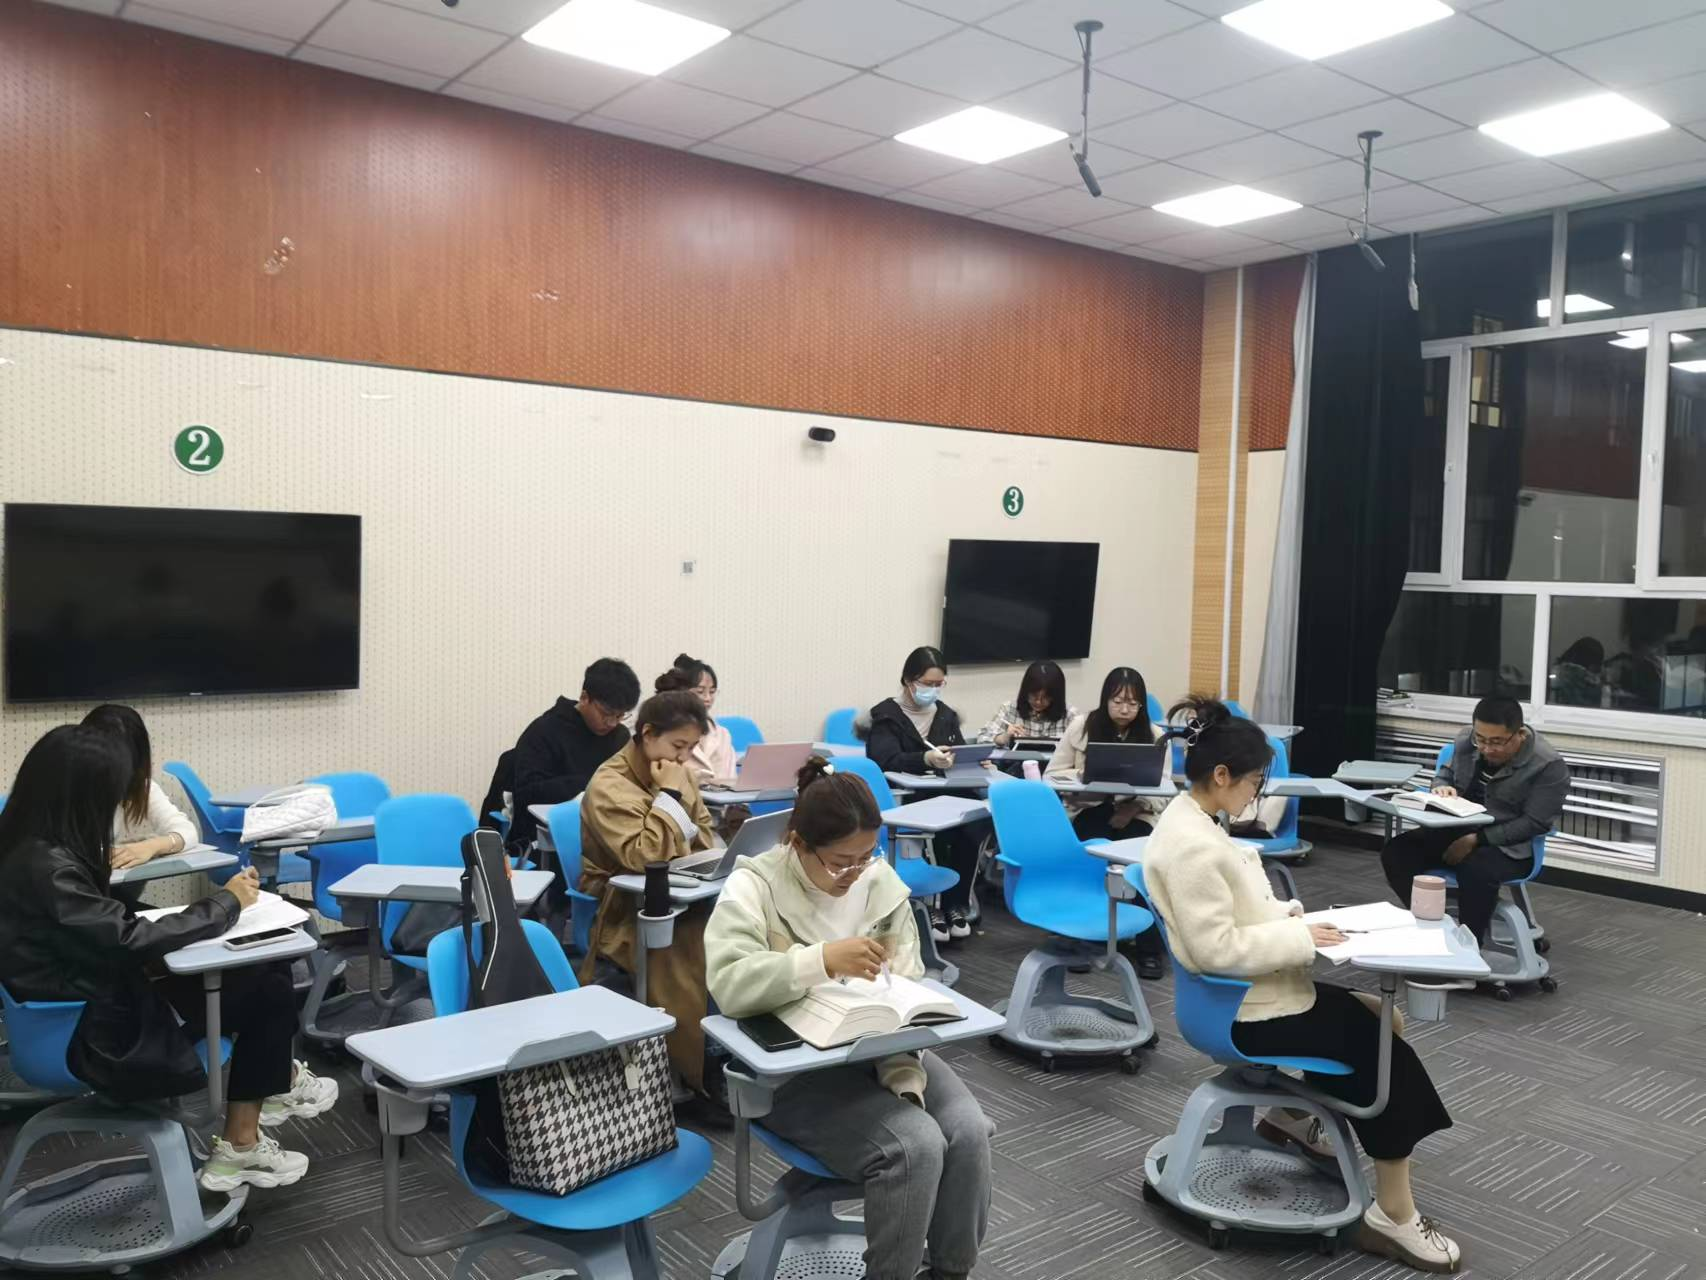
\includegraphics[width=1\linewidth]{10.23.jpg}
    \caption{第二期读书会实拍图(2023.10.23)}
    \label{fig1}
\end{figure}
2023年10月23日18:00—20:00,我们在东北林业大学奥林学院203教室开展了第二期的读书会。本期读书会我们阅读了《哲学的贫困》第二章第一节中的\textbf{“第五个说明”}与\textbf{“第六个说明”}。我们本期做了非常丰富的讨论,现场情况见\textbf{\nameref{fig1}}\footnote{在这里非常抱歉,由于本期读书会讨论的过于热情,以至于我在中途拍照的时候漏掉了一些同学与老师。},主要讨论内容可简要地概括如下:
\subsubsection{1.第五个说明}

在“第五个说明”中,马克思首先指出:
\begin{adjustwidth}{2em}{2em}
    \qquad\fangsong
    “如果把辩证运动的全部过程归结为简单地对比善和恶,归结为提出任务来消除恶并且把一个范畴用作另一个范畴的消毒剂,那末范畴就失去自己的独立运动;观念就“不再发生作用”;他就没有内在的生命。它既不能把自己安置为范畴,也不能把自己分解为范畴。范畴的顺序成了一种脚手架。辩证法已不是绝对理性的运动了。辩证法没有了,代替它的至多不过是最纯粹的道德而已。”
\end{adjustwidth}

这里马克思似乎是想表达:“辨证运动”并不是蒲鲁东所认为的那种“简单地对比善和恶,并提出任务来消除恶”。马克思认为蒲鲁东的“辩证运动”不过是借助他自己的搭建出的一种“脚手架”而进行的,这意味着蒲鲁东将黑格尔所认为的“范畴的自我运动”变成了通过他(指蒲鲁东)自己搭建起来的“脚手架”而进行的运动。因此,马克思会说,在蒲鲁东的“辩证运动”下,范畴本身“就没有内在的生命”了。

之后,马克思揭示了蒲鲁东自己的逻辑混乱。马克思认为,蒲鲁东在谈论“历史”的时候,他是从他自认为的“范畴的顺序”\footnote{根据前文的分析,不难理解,这种“范畴的顺序”是通过蒲鲁东自己构建的“脚手架”而展开的。}去出发的。但是,当蒲鲁东将他自认为的“范畴的顺序”应用到现实中时,便同现实产生了矛盾。因此马克思指出:
\begin{adjustwidth}{2em}{2em}
    \qquad\fangsong
    “……于是蒲鲁东先生只得承认,他用以说明经济范畴的次序和这些经济范畴在其中相互产生的次序是不相适应的。经济的进化不再是理性本身的进化了。”
\end{adjustwidth}

最后,马克思在“第五个说明”中的最后一部分的内容中强调,如果按照蒲鲁东所设想的“现实的历史是观念、范畴和原理在其中出现的那种历史顺序”的话,那末就必须对此进行进一步的追问。也即是说,如果说是某一时代的原理创造了这一时代的历史的话,那末,为什么这一时代的原理没有创造别的时代的历史呢?为什么这一时代的原理恰好地就出现在这一时代了呢?为了回答上述疑问,就必须进一步考察那一时代的人们是怎样进行生产生活的、那一时代的人们之间的关系是怎么样的。但只要进入到对具体时代的人们的生产生活的考察之中,那末就是背弃了那种认为“观念创造历史”的观点,就是回到了历史发生的真正出发点。

因此,马克思在最后是这么论述的:
\begin{adjustwidth}{2em}{2em}
    \qquad\fangsong
“我们暂且和蒲鲁东先生一同假定:现实的历史,适应时间次序的历史是观念、范畴和原理在其中出现的那种历史顺序。

每个原理都有其出现的世纪。例如,与权威原理相适应的是11世纪,与个人主义原理相适应的是18世纪,推其因果,我们应当说,不是原理属于世纪,而是世纪属于原理。换句话说,不是历史创造原理,而是原理创造历史。但是,如果为了顾全原理和历史我们再进一步自问一下,为什么该原理出现在11世纪或者18世纪,而不出现在其它某一世纪,我们就必然要仔细研究一下:11世纪的人们是怎样的,18世纪的人们是怎样的,在每个世纪中,人们的需求、生产力、生产方式以及生产中使用的原料是怎样的;最后,由这一切生存条件所产生的人与人之间的关系是怎样的。难道探讨这一切问题不就是研究每个世纪中人们的现实的、世俗的历史,不就是把这些人既当成剧作者又当成剧中人物吗?但是,只要你们把人们当成他们本身历史的剧中人物和剧作者,你们就是迂回曲折地回到真正的出发点,因为你们抛弃了最初作为出发点的永恒的原理。”
\end{adjustwidth}

\subsubsection{2.第六个说明}
马克思在这部分内容中开篇提到:
\begin{adjustwidth}{2em}{2em}
    \qquad\fangsong
    “我们已经看到,在这一切一成不变的、停滞不动的永恒下面没有历史可言,即使有,至多也只是观念中的历史,即反映在纯理性的辩证运动中的历史。蒲鲁东先生谈到辩证运动中的各种观念不能自相‘区分’时,把运动的一切影子和影子(它们可以造成某种类似历史的东西)的一切运动一概抹熬。”
\end{adjustwidth}

其中,\textbf{“运动的影子”}和\textbf{“影子的运动”}分别代表的是什么意思呢?在这里,我们认为前者指的是“感性历史”的理论表现,后者指的是黑格尔的那种“纯粹理性”的运动。因此,我们可以认为,马克思在这里想表明:蒲鲁东所谈论的“辨证运动”既不是对感性历史发展过程的理论表达,也不是对黑格尔式的纯粹理性的运动的表达。因此,正如前面我们所讨论的那样,事实上,蒲鲁东自己构建了一个范畴的“脚手架”,范畴遵循着蒲鲁东自己构建的“脚手架”向上爬行。而范畴为什么要踏着“脚手架”向上运动呢?因为蒲鲁东认为范畴就得踏着他所构建的“脚手架”向上运动,这似乎是蒲鲁东先生的一厢情愿。

既然蒲鲁东的“辨证运动”既不是对感性历史的理论表达,也不是对黑格尔式的“纯粹理性”运动的表达,那末,蒲鲁东是如何从底层逻辑层面说明他的“辩证运动”的合理性的呢?很简单,既然蒲鲁东自己的“辨证运动”既不是“运动的影子”也不是“影子的运动”,那末,蒲鲁东先生完全可以“大言不惭地”构建出一个新的规律,并用一种“唬人的词句”宣称这种规律的至高性地位。因此,蒲鲁东先生自己构建出了所谓的\textbf{“人类理性”}、\textbf{“社会天才”}等等的概念。然而事实上,我们不难看出,所谓的\textbf{“人类理性”}、\textbf{“社会天才”}等的概念不过是蒲鲁东自己虚构出来的东西,不过是蒲鲁东自己的主观设想。

因此,当蒲鲁东的理论同现实的历史之间发生矛盾的时候,他就将这些\textbf{“矛盾”}看作是\textbf{“人类理性”}、\textbf{“社会天才”}的任务,他认为\textbf{“人类理性”}、\textbf{“社会天才”}就是需要解决这些矛盾的,进而使得范畴朝着\textbf{“人类理性”}、\textbf{“社会天才”}所期待的目标发展。

因而我个人\footnote{指本书编者。}认为,在马克思的视角下,蒲鲁东的逻辑进路应可分为如下的步骤:


\begin{tcolorbox}[colback=gray!20, colframe=gray!100, sharp corners, leftrule={3pt}, rightrule={0pt}, toprule={0pt}, bottomrule={0pt}, left={2pt}, right={2pt}, top={3pt}, bottom={3pt}] 
\textbf{step1.}假定有一个“先在”的真理:例如“纯粹的平等”、“纯粹的自由”等最终的概念。

\textbf{step2.}假定一种“规则”:可以通过这种“规则”发现“真理”,并把这种“规则”命名为“人类理性”、“社会天才”。

\textbf{step3.}因此,当理论同现实相违背时,蒲鲁东就可以借着“人类理性”、“社会天才”的名义说:这种矛盾正是要通过“辩证运动”被解决的!


\end{tcolorbox}

因此,马克思会说:
\begin{adjustwidth}{2em}{2em}
    \qquad\fangsong
    “假设只是为了某种特定的目的而设立的。通过蒲鲁东先生之口讲话的社会天才首先给自己提出的目的,就是消除每个经济范畴的一切坏的东西,使它只保留好的东西。他认为,好的东西,最高的幸福,真正的实际目的就是平等。为什么社会天才只要平等,而不要不平等或友爱、不要天主教或别的什么原理呢?因为‘人类之所以实现这么多特殊的假设,正是由于考虑到一个最高的假设’,这个最高的假设就是平等。换句话说,因为平等是蒲鲁东先生的理想。他以为分工、信用、工厂,一句话,一切经济关系都仅仅是为了平等的利益才被发明的,但是结果它们往往对平等不利。由于历史和蒲鲁东先生的臆测步步发生矛盾,所以他得出结论说,有矛盾存在。即使是有矛盾存在,那也只存在于他的固定观念和现实运动之间。”
\end{adjustwidth}

在上面马克思的这段论述中,我们可以挑几句关键的句子来看,例如:\begin{fangsong}
    “通过蒲鲁东之口讲话的社会天才”
\end{fangsong},以及\begin{fangsong}
    “为什么社会天才只要平等,而不要不平等或友爱、不要天主教或别的什么原理呢?……因为平等是蒲鲁东先生的理想”
\end{fangsong}
等。不难看出,前面这几句话处处体现出了我在前文所概括的\textbf{“蒲鲁东的逻辑进路”}中的三个步骤。因此,马克思会指出:\begin{fangsong}
    “即使是有矛盾存在,那也只存在于他<指蒲鲁东>\footnote{编者注。}的固定观念和现实运动之间。”
\end{fangsong}

因此我们可以看到,马克思在这里最终想要表达的是:\textbf{蒲鲁东的思想既不唯物,也不客观。}在这里,我个人\footnote{指本书编者。}认为,蒲鲁东的思想既没有超越古典经济学家们,也没有超越黑格尔。因为,相较于古典经济学家们而言,蒲鲁东缺少了这些理论家们的唯物主义倾向;相较于黑格尔而言,蒲鲁东也没有领悟“辩证法”或“辨证运动”的实质,因而蒲鲁东的思想更像一种拙劣的“折衷主义”\footnote{事实上,我认为在“第七个说明”中马克思对蒲鲁东的这种“折衷主义”的批判会体现地更为明显,但本期讨论会并没有讨论到“第七个说明”,因此这里先按下不表。}。

在“第六个说明”的最后,马克思这样说道:
\begin{adjustwidth}{2em}{2em}
    \qquad\fangsong
    “当然,平等趋势是我们这个世纪所特有的。但是,说以往各世纪及其完全不同的需求、生产资料等等都是为实现平等而遵照天命行事,这首先就是把我们这个世纪的人和生产资料当做过去世纪的人和生产资料看待,否认世世代代不断改变前代所获得的成果的历史运动。经济学家们很清楚,同是一件东西对甲说来是成品,对乙说来只是从事另一种生产的原料。
    
    如果你们同蒲鲁东先生一道假定:社会天才制造出,或者更确切些说随兴制造出封建主,是为了达到把耕者变为负有义务的和彼此平等的劳动者这一天命的目的,那末,你们就是把目的和人换了一下,这种做法和为了达到恶意的满足(即羊群赶走人)而在苏格兰确立土地私有制的天命比较起来,毫不逊色。”
\end{adjustwidth}

马克思这两段论述同样地体现出了满满的历史唯物主义原则。马克思承认,“平等”确实是当时那个世纪所特有的思想倾向,但他想进一步表明的是,并不是自古以来就一直存在着这种“平等”的思想倾向的。如果将“平等”这种仅仅在当时那个世纪所特有的思想倾向看作是永恒不变的思想倾向的话,就意味着,当时那个世纪的人的物质生产活动同以往一切世纪的物质生产活动之间并无差别了。而这种观念是反历史唯物主义的,在这里就不赘述了。

\subsubsection{本期小结:以及一些余论}
本期我们讨论的比较热烈,同时一些新同学也在本期加入了我们的讨论会。在本期讨论会的最后几分钟,我们初步探讨了一下古典国民经济学(特别是李嘉图的经济学)同马克思主义经济学之间的差异。我们探讨了“李嘉图难题”的产生,以及马克思是如何解决李嘉图难题的(但我们只是初步地提了一嘴,并没有深入讨论下去)。我们计划在下期的讨论会中留一段时间和大家讨论一下李嘉图的利润理论与马克思之间的差异,以及马克思是如何系统地批判李嘉图经济学的。总之,这是一期收获很满的讨论会。



\end{document}
